\section{System description}

\subsection{Overview}

\begin{figure}[ht!]
\centering
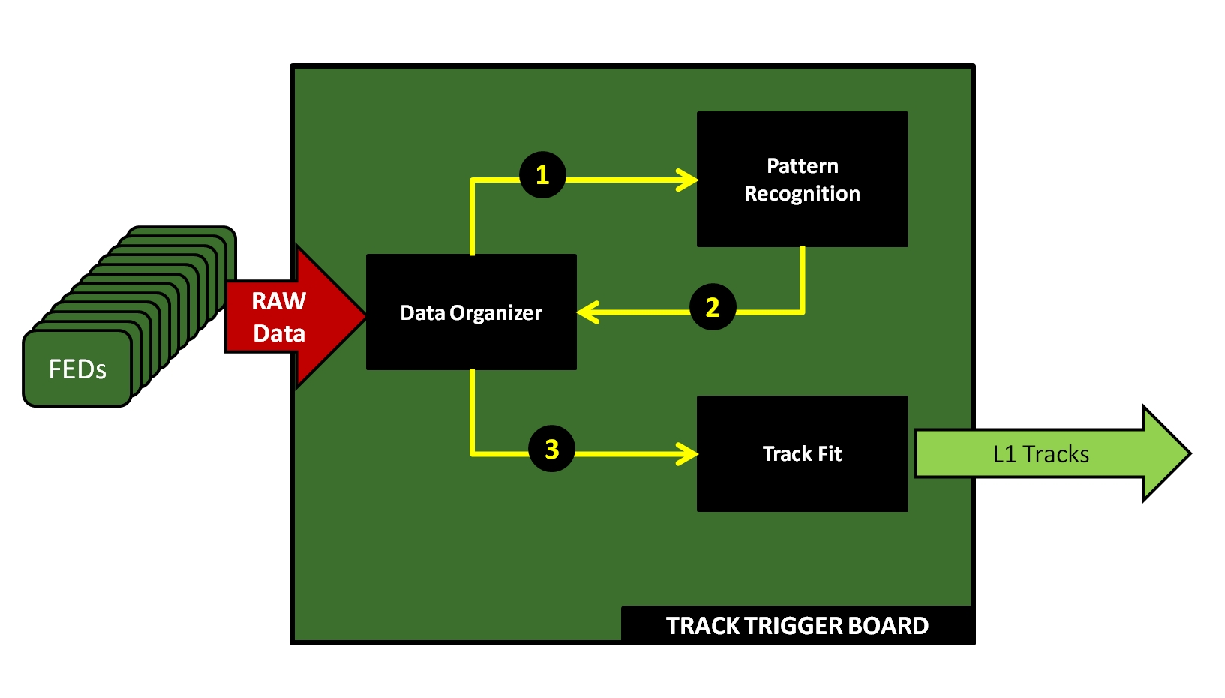
\includegraphics[width=0.5\columnwidth]{Plots/L1TTrigPrinciple.eps}
\caption{Hardware tracking principle}
\label{fig:L1TT_principle}
\end{figure}

\noindent Extracting track information is a two-stage process. First of all, you have to retrieve the hits belonging to the track: this is the pattern recognition. Then, you extract the track parameters (momentum, impact parameter,...) from the hits: this is the fit. Both steps are performed routinely in CMS, using very performant software algorithms. In order to pass to L1, tracking has to go hardware. Hardware-based tracking triggers were already developped in HEP experiments, in particular in the CDF experiment at Fermilab. Based on this system, the ATLAS experiment is planning to use a tracking trigger at the HLT after LHC long shutdown 2 in 2016. The working principle of these systems is sketched on Fig.~\ref{fig:L1TT_principle}. Tracker data is extracted by the FEDs and transmitted to the trigger board. Then, the data is handled by a data organization unit (DO), which extract the info necessary to the pattern recognition (PR), send it to the PR unit, and retrieve the matched patterns. The DO then sent the interesting hits to the track fit unit (TF), when the track parameters are estimated and sent to the L1 central trigger board.
\noindent In order to go at L1, one thus need the three following points: 

\begin{itemize}
\item A fast front-end readout system able to extract quickly all the data contained in the tracking detectors.
\item A system performing a fast pattern recognition.
\item A system performing a fast track fit.
\end{itemize}

\noindent Using associative memories in order to perform a fast pattern recognition (PR) at the trigger stage was first exposed in Ref.~\cite{bib:Del-89}. The principle is sketched in Fig.~\cite{fig:AM_principle}:
\begin{figure}[ht!]
\centering
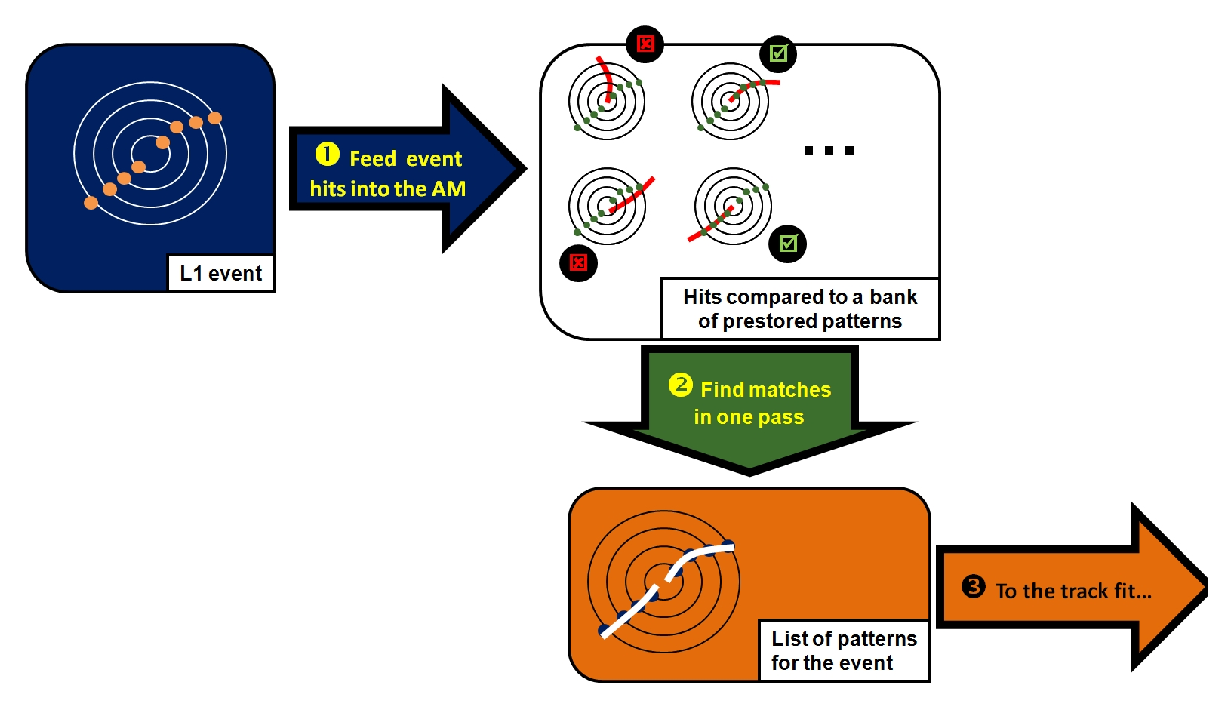
\includegraphics[width=0.7\columnwidth]{Plots/TriggerAM.eps}
\caption{Pattern recognition using associative memories.}
\label{fig:AM_principle}
\end{figure}

\noindent The idea is to compare the hits recorded in the tracking system to a bank of patterns stored in an associative memory chip. The patterns could be seen as low-granularity tracks, they are defined once for all using Monte-Carlo events, and they are ideally covering all the possible tracks occuring in the detector. In this part we will concentrate ourselves on the pattern bank definition. This is indeed the central point of the PR stage. The bank, which is defined using simulated events, has to fulfill few requirements. Before presenting them, it's important to define some parameters. 

\subsection{Data flow}

\subsection{Interface with Tracker FEDs and L1 Global Trigger}

\subsection{Simulation tools and needs}


\clearpage
